\chapter{Sistema Acadêmico Minha Uno}

Desenvolvido pela Unochapecó, o sistema acadêmico “Minha Uno'' é a interface utilizada pelos acadêmicos, docentes e funcionários da universidade para envio e recebimento de informações.

O sistema consiste em uma página web, dividida em perfis, com opções diferentes para cada um deles. O sistema é composto pelos perfis “Graduação'', “Pós-Graduação'', “Professor'', “Técnico-Administrativo'', “Administrador'', “Fornecedor'' e “Apoio-Operacional''.

Dentre os perfis existentes no sistema, foram avaliados os perfis: Professor, Graduação, Pós-Graduação e Técnico-Administrativo.


\section{Graduação}
O perfil de graduação é voltado aos acadêmicos dos diferentes cursos da Unochapecó. Por meio dele, 
os acadêmicos são informados das  suas notas, recebem novos materiais, 
se informam da sua situação financeira, solicitam documentos entre outras opções.

Com uma interface confusa em alguns momentos, porém de modo geral de fácil aprendizado, 
a mesma é de uso obrigatório para qualquer graduando da instituição, pois sem ela não é possível 
acompanhar as notas, entregar alguns trabalhos ou tirar os boletos para o pagamento das mensalidades. 
Abaixo lista completa das opções fornecidas por este perfil: \\
- Atividades Curriculares Complementares \\
- Bolsa de Estudo \\
- Bolsa de Pesquisa \\
- Cadastro de Objetos Pedidos \\
- Componentes Curriculares Fora da Matriz \\
- Componentes Curriculares Isolados \\
- Componentes Curriculares Turno Diferenciado \\
- Conhecimento Prévio \\
- Disponibilidade de Laboratórios de Informática \\
- Dúvidas/Sugestões \\
- E-mail \\
- Entrega de Trabalhos \\
- Ficha de Matrícula \\
- Financiamento \\
- Formulário para Negociação Diferenciada \\
- Histórico \\
- Horários de Aula/Ementas/Requisitos \\
- Horários do Semestre \\
- Inscrições em Eventos \\
- Inscrições para Estágio \\
- Material de Apoio/Planos de Ensino \\
- Negociação pela Internet \\
- Notas Graduação \\
- Pedidos de Livros Livraria Universitária \\
- Programa de Incentivos \\
- Protocolo Digital \\
- Quero Livro - Curso de Direito \\
- Renovação de Matricula \\
- Situação Financeira \\
- Solicitação de Documentos \\
- Solicitação de Estágio - Cursos de Direito e Farmácia \\
- Titulos a Receber e \\
- Trancamento parcial. \\

O layout do sistema acadêmico e a disposição dos itens pode ser visualizado na Figura 1.

\begin{figure}[!htb]
     \centering
     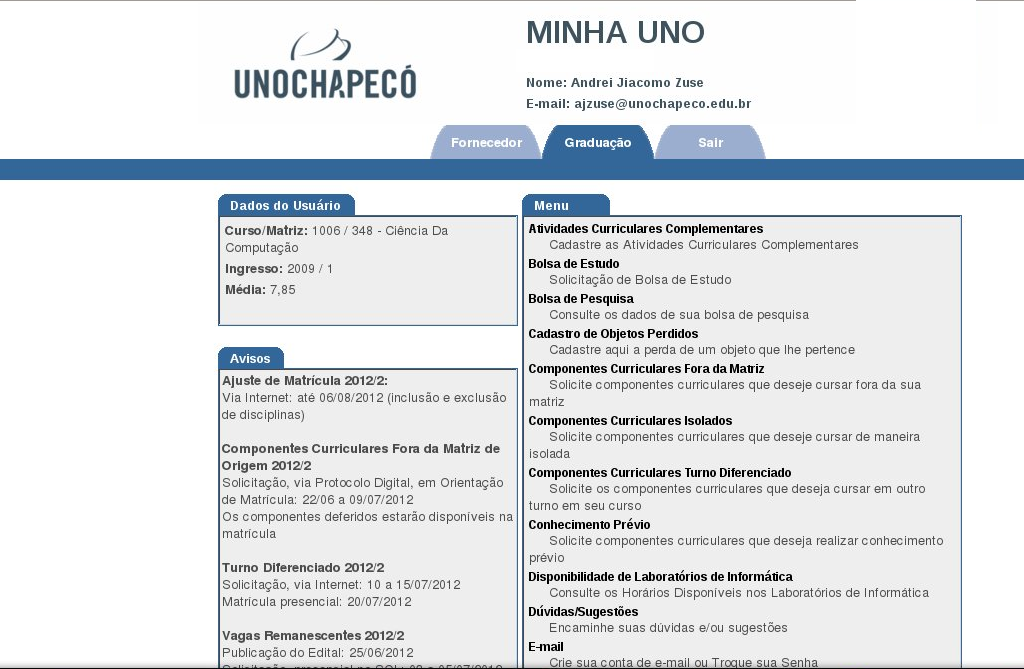
\includegraphics[scale=0.3]{imagens/GraduacaoCorrigida.png}
     \caption[Layout do Sistema - Perfil Graduação]{Layout do perfil Graduação do Sistema Acadêmico Minha Uno. Fonte: Do Autor}
\end{figure}

\newpage
\section{Pós-Graduação}
O perfil de pós-graduação é voltado aos acadêmicos dos diferentes cursos de pós-graduação da Unochapecó. 
Por meio dele, os acadêmicos são informados das  suas notas, recebem novos materiais, 
se informam da sua situação financeira, solicitam documentos entre outras opções.

Com uma interface mais limpa que a apresentada pelo perfil de graduação, a mesma é de uso obrigatório para qualquer 
pós-graduando da instituição, pois sem ela não é possível acompanhar as notas, entregar alguns trabalhos ou 
tirar os boletos para o pagamento das mensalidades. As opções presentes neste perfil são: \\
- Cadastro de Objetos Perdidos; \\
- Dúvidas/Sugestões \\
- E-mail \\
- Ementas \\
- Entrega de Trabalhos \\
- Inscrições em Eventos \\
- Material de Apoio/Planosd e Ensino \\
- Notas Pós-Graduação \\
- Pedidos de Livros Livraria Universitária \\
- Programa de Incentivos \\
- Protocolo Digital \\
- Situação Financeira \\
- Solicitação de Documentos e \\
- Títulos a Receber. \\

O layout do sistema acadêmico e a disposição dos itens pode ser visualizado na Figura 2.

\begin{figure}[!htb]
     \centering
     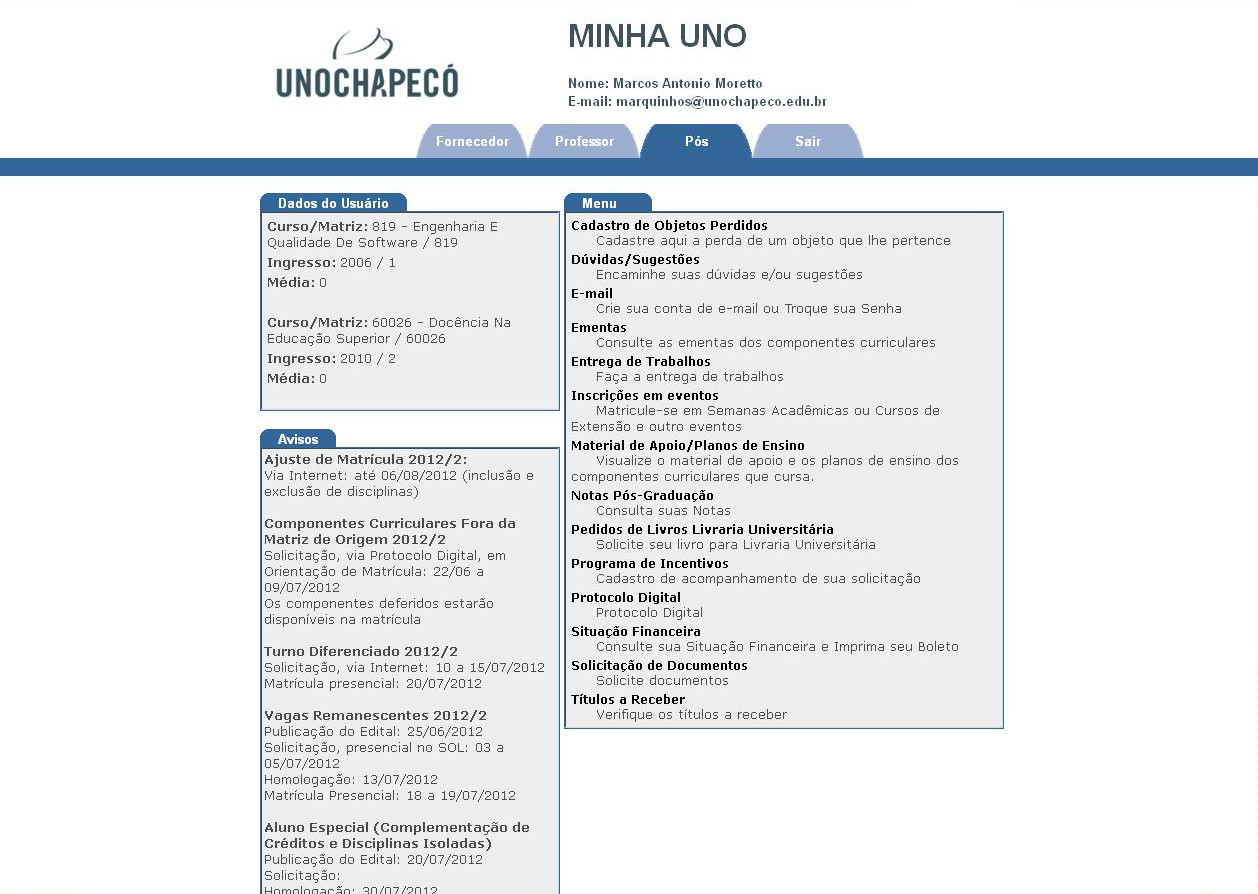
\includegraphics[scale=0.3]{imagens/pos.jpg}
     \caption[Layout do Sistema - Perfil Pós-Graduação]{Layout do perfil Pós-Graduação do Sistema Acadêmico Minha Uno. Fonte: Do Autor}
\end{figure}

\section{Professor}
Utilizado pelos docentes da instituição, o perfil de Professor pode ser considerado o painel de controle das disciplinas
ministradas. Utilizando-se do perfil no Sistema Acadêmico o professor coloca novos materiais nas disciplinas ministradas,
adiciona as notas dos alunos, envia mensagens aos mesmos, efetua as chamadas entre outras funcionalidades.
As opções disponíveis neste perfil são: \\
- Cadastro de Objetos Perdidos \\
- Cadastro de Veículo \\
- Componentes Curriculares Complementares \\
- Comunicação Interna Eletrônica \\
- Contato RH \\
- Diário de Classe On-Line \\
- Documentos Diversos \\
- E-mail \\
- Entrega de Trabalhos \\
- Envio de Projetos de Pesquisa \\
- Folha de Pagamento \\
- Gastos dos Convênios Asser \\
- Horários de Aula/Ementas/Requisitos \\
- Horários do Professor \\
- Inscrições em Eventos \\
- Ligações Telefônicas \\
- Material de Apoio \\
- Pedidos de Livros Livraria Universitária \\
- Período de Férias \\
- Plano de Ensino \\
- Plano Mensal de Trabalho do Professor \\
- Processo Seletivo \\
- Programa de Aprendizagem \\
- Quero Livro - Curso de Direito \\
- Ramais \\
- Registro das Atividades Mensais \\
- Relatório on-line/Projetos de pesquisa \\
- Repositório de Arquivos \\
- Reservas \\
- Reservas Laboratório de Informática \\
- Sistema de Mensagem Integrada \\
- Solicitação de Coffee Break e \\
- Sumula de Currículo. \\

O layout do sistema acadêmico e a disposição dos itens pode ser visualizado na Figura 3.


\begin{figure}[!htb]
     \centering
     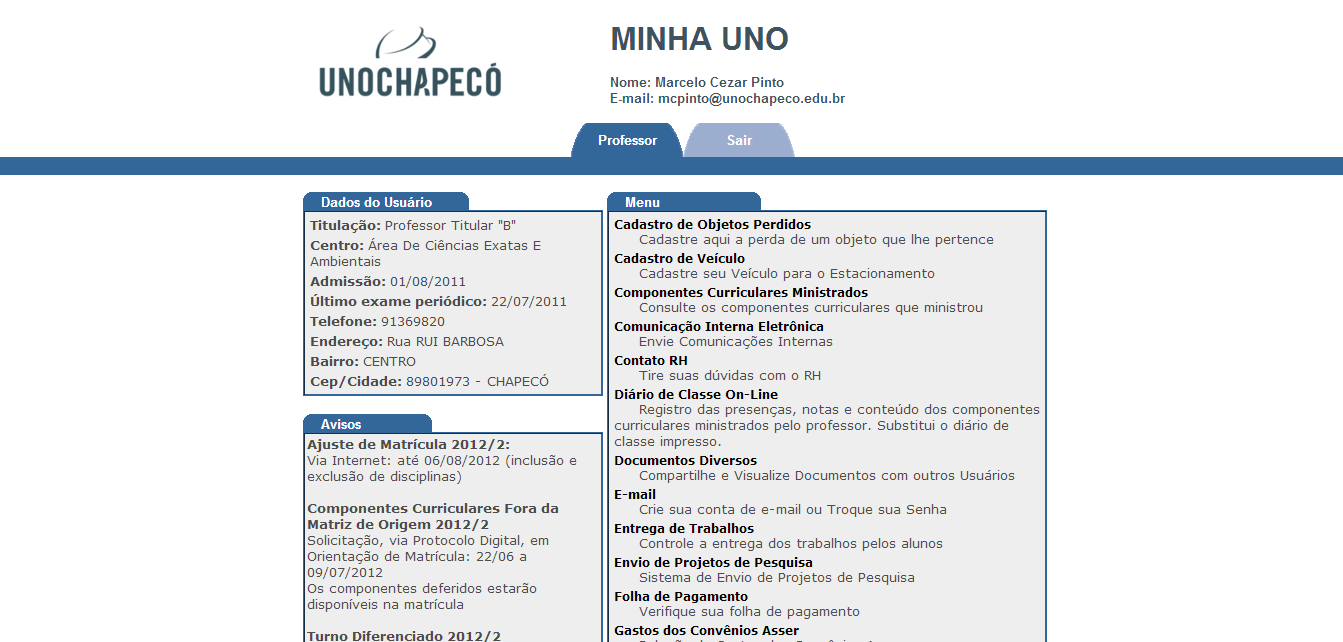
\includegraphics[scale=0.4]{imagens/professor.png}
     \caption[Layout do Sistema - Perfil Professor]{Layout do perfil Professor do Sistema Acadêmico Minha Uno. Fonte: Do Autor}
\end{figure}

\newpage

\section{Técnico-Administrativo}
Utilizado pelos Funcionários da Unochapecó para comunicação interna, entrar em contato com o setor de Recursos Humanos (RH),
consultar sua folha de pagamento, participar de processos seletivos entre outras tarefas, o perfil Técnico-Administrativo
possui as seguintes opções: \\
- Cadastro de Artigos/Monografias/TCC \\
- Cadastro de Objetos Perdidos \\
- Cadastro de Veículo \\
- Cartão-Ponto \\
- Comunicação Interna Eletrônica \\
- Contato RH \\
- Documentos Diversos \\
- E-mail \\
- Folha de Pagamento \\
- Gastos dos Convênios Asser \\
- Inscrições em Eventos \\
- Ligações Telefônicas \\
- Pedidos de Livros Livraria Universitária
- Período de Férias \\
- Processo Seletivo \\
- Ramais \\
- Repositório de Arquivos \\
- Reservas \\
- Reservas Laboratório de Informática \\
- Sistema de Mensagem Integrada \\
- Solicitação de Coffee Break \\
- Sumula de Currículo e \\
- Títulos a Receber. \\

O layout do sistema acadêmico e a disposição dos itens pode ser visualizado na Figura 1.


\begin{figure}[!htb]
     \centering
     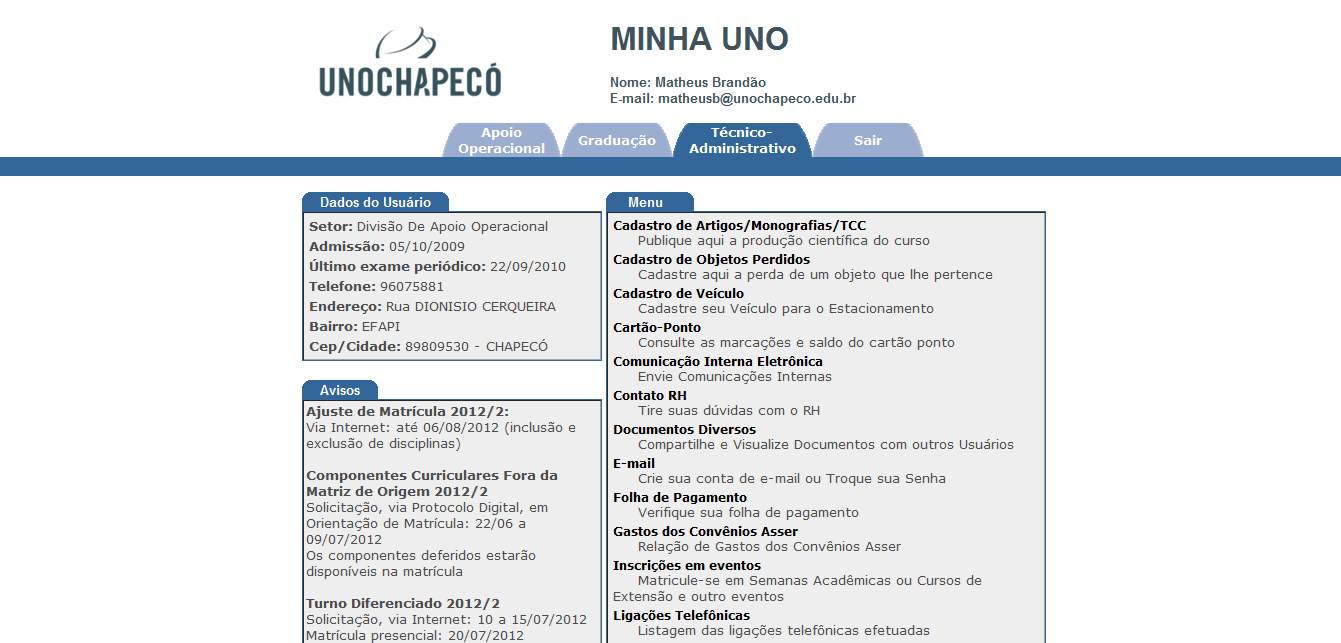
\includegraphics[scale=0.4]{imagens/tecnico.png}
     \caption[Layout do Sistema - Perfil Técnico-Administrativo]{Layout do perfil Técnico-Administrativo do Sistema Acadêmico Minha Uno. Fonte: Do Autor}
\end{figure}